\obcfunc{Boot loading}
\subsection{Boot table layout}
Boot table contains following elements:
\begin{itemize}
	\item 6 boot slots with OBC program and metadata (CRC, description, valid flag)
	\item 5 bootloader copies
	\item 5 safe mode copies
\end{itemize}

Figure \ref{fig:func:boottable} shows boot table layout inside memory.

\begin{figure}
	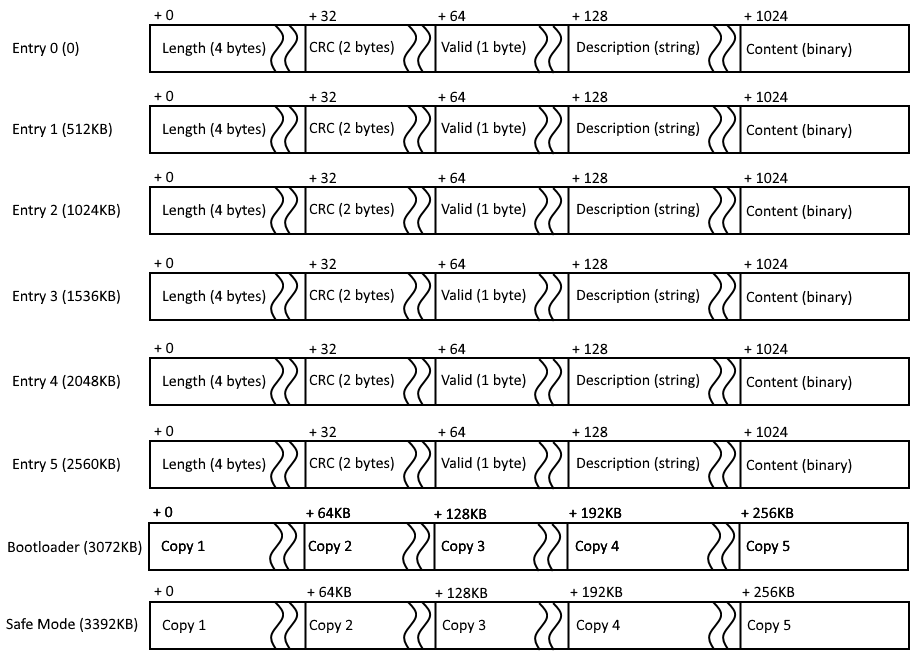
\includegraphics[width=20cm,angle=90]{img/boot-table.png}
	\caption{Boot table layout}
	\label{fig:func:boottable}
\end{figure}

\subsection{Boot configuration}
There are 4 settings in \nameref{obc:proc:Persistent State} related to boot process:
\begin{itemize}
	\item Primary boot slots
	\item Failsafe boot slots
	\item Boot counter
	\item Last confirmed boot counter
\end{itemize}

Primary and failsafe boot slots are bitmasks indicating three boot entries used to boot main OBC program. For example: binary value \texttt{00010101} represents boot slots 0, 2, 5. In addition there are two special values:
\begin{itemize}
	\item \texttt{01000000} - Safe mode
	\item \texttt{10000000} - OBC main without refreshing from boot slots
\end{itemize}

Boot counters are used to detect main OBC program that is failing to boot. Two counters are used: 
\begin{itemize}
	\item \texttt{BootCounter} - incremented on every boot before transfering control to main OBC program.
	\item \texttt{LastConfirmedBootCounter} - set to the value of \texttt{BootCounter} after main OBC program claims successful boot.
\end{itemize}

In normal conditions these counters should be equal. If difference between \texttt{BootCounter} and \texttt{LastConfirmedBootCounter} is greater or equal to 10, bootloader treats that situation as invalid program in primary boot slots and attempts boot from failsafe boot slots. If it also fails, safe mode is triggered.

\subsection{Boot procedure}
Boot procedure is multi-step process divided between main OBC program and bootloader.

\subsubsection{Bootloader}
\begin{enumerate}
	\item If difference between \texttt{BootCounter} and \texttt{LastConfirmedBootCounter} is greater or equal to 10 and primary boot slots are already set to failsafe boot slots, boot to safe mode (and stop this procedure)
	\item If difference between \texttt{BootCounter} and \texttt{LastConfirmedBootCounter} is greater or equal to 10, switch primary boot slots to failsafe boot slots
	\item Increment boot counter
	\item Load main OBC program using TMR on selected boot slots
	\item Enable 16 seconds watchdog
	\item Transfer control to main OBC program
\end{enumerate}

\subsubsection{Main OBC program}
\begin{enumerate}
	\item Disable watchdog
	\item Initialize hardware 
	\item Initialize file system
	\item Start mission and telemetry loop
	\item Claim correct boot (set \texttt{LastConfirmedBootCounter} to be equal with \texttt{BootCounter})
\end{enumerate}

Whole OBC boot procedure can take up to \textbf{5 minutes}. 

\subsection{Safe mode}
Safe-mode is everything-gone-shit-program trigged when bootloader is unable to boot any program (from primary and failsafe boot slots). Recovery is performed by executing following steps:
\begin{enumerate}
	\item Scrubs bootloader
	\item Scrubs boot slots using TMR on slots 0,1,2 and 3,4,5
	\item Erases flash-storage
	\item Reset bootslots to default (primary - 0,1,2 failsafe - 3,4,5)
	\item Reboots
\end{enumerate}

Safe mode will keep mission time but erase all telemetry and experiment data. 

\danger{Using not standard boot slots configuration will result in very fast moving brick as OBC will not be able to boot again.}

\subsection{Periodic restart}
Restart after 23 hours of mission time since last boot according to \nameref{obc:proc:Power cycle}. 
